For a successful system installation the following elements are required:


\begin{itemize}
	\item \textbf{Installation scripts}.  To facilitate the installation task, and since this system has multiple internal and third-party components,  the developers have created a series of scripts that automate the system installation.
	\item \textit{GNU/Linux distribution}.  The installation scripts have been only tested under Ubuntu 14.04 LTS, so it is highly recommended to use this distribution for the system deployment.
\end{itemize}

The first step consists of logging into the system with a non-root account.  The non-root account is important because the file paths in the scripts are relative to the user's home directory, the root home directory is \textit{/root} while the home directory for regular users is \textit{/home/USERNAME}.

Once you have logged into the system with a non-root account, the following step consists of copying the content of the scripts folder into the user's home directory.  Such as in the image \ref{fig:manual_instalacion_home}, the files \textit{install.sh} and \textit{settings.ph} and the folders \textit{scripts} and \textins{solr} must be located into the root of the user's home directory.

\begin{figure}[h]
	\centering
	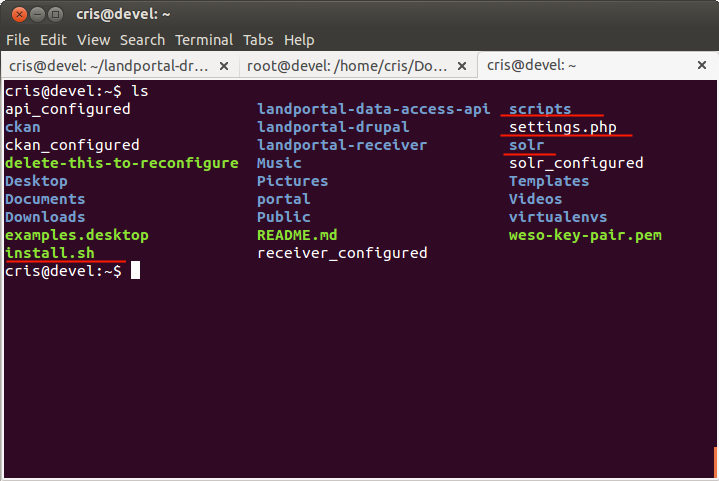
\includegraphics[width=\textwidth]{manual_instalacion/home_folder}
	\caption{User's home folder with the script files (underlined in red)}
	\label{fig:manual_instalacion_home}
\end{figure}

After copying the installation scripts into the home directory, the system installation can be easily triggered with the command \textit{sudo ./install.sh}, which means to run the script \textit{install.sh}, which is located into the current directory, with superuser privileges.  The superuser privileges are required to install some packages and configurations.  The image \ref{fig:manual_instalacion_lanzamiento} shows the command before starting the installation.

When you hit the \textit{enter} key, the installation will begin.  The installation process is completely automated and requires no user interaction, but since it is such a big system, the installation can last a long time.

After the installation ends, the system is completely functional, but it still needs some configuration.  Please, take a look into the ``\nameref{anexo_manual_configuracion}''.

\begin{figure}[h]
	\centering
	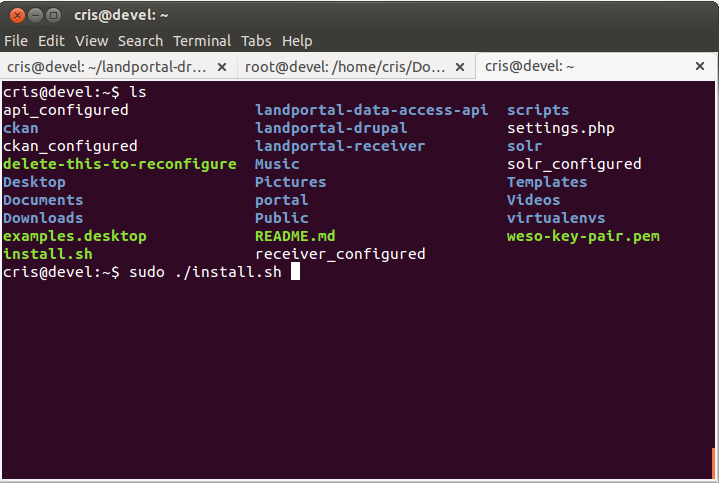
\includegraphics[width=\textwidth]{manual_instalacion/launch_installation}
	\caption{Launch system installation command}
	\label{fig:manual_instalacion_lanzamiento}
\end{figure}